\chapter{Практическая часть}

Для первого и второго задания был написан обработчик прерывания для irq = 1.

\section{Задание 1}
На листинге ниже представлен текст программы первого задания.

\lstset{language=c}
\begin{lstlisting}[caption=Текст программы]
#include <linux/module.h>
#include <linux/kernel.h>
#include <linux/init.h>
#include <linux/interrupt.h>
#include <linux/time.h>

MODULE_AUTHOR("Alexander Kupry");
MODULE_LICENSE("GPL");
MODULE_DESCRIPTION("lab_09_task_1");

#define HANDLEDIRQ 1

static int irq = HANDLEDIRQ;
static int irq_call_count = 0;
static int dev_id;

void tasklet_function(unsigned long data);

char tasklet_data[] = "tasklet_function was called";
DECLARE_TASKLET(tasklet, tasklet_function, (unsigned long)&tasklet_data);

void tasklet_function(unsigned long data)
{
    struct timeval t;
    struct tm brocken;
    do_gettimeofday(&t);
    time_to_tm(t.tv_sec, 0, &brocken);

    printk(KERN_INFO "TASKLET MODULE\nTasklet: { state: %ld, count: %d, data: %s }, current_time: %d:%d:%d:%ld\n",
        tasklet.state, atomic_read(&tasklet.count), (char *)tasklet.data,
        brocken.tm_hour + 3, brocken.tm_min, brocken.tm_sec, t.tv_usec);
}

static irqreturn_t interrupt_handler(int irq, void *dev_id)
{
    if (irq == HANDLEDIRQ)
    {
        irq_call_count++;
        printk(KERN_INFO "TASKLET MODULE\nirq call count = %d\n", irq_call_count);
        tasklet_schedule(&tasklet);
        return IRQ_HANDLED;
    }
    else
    {
        return IRQ_NONE;
    }
}

static int __init tasklet_module_init(void)
{
    int ret = request_irq(irq, interrupt_handler, IRQF_SHARED, "tasklet_interrupt_handler", &dev_id);

    if (ret)
    {
        printk(KERN_ERR "TASKLET MODULE\nerror while handle irq\n");
        return -1;
    }

    printk(KERN_INFO "TASKLET MODULE\nsuccess load\n");
    return 0;
}

static void __exit tasklet_module_exit(void)
{
    tasklet_kill(&tasklet);
    free_irq(irq, &dev_id);
    printk(KERN_INFO "TASKLET MODULE\nunload module\n");
}

module_init(tasklet_module_init);
module_exit(tasklet_module_exit);
\end{lstlisting}

Компиляция загружаемого модуля ядра при помощи Makefile:
\begin{figure}[H]
    \centering
    \includegraphics[scale=0.3]{data/image/make_tasklet.png}
    \caption{Скришот результата работы make.}
\end{figure}

Загрузка модуля ядра с помощью команды insmod:
\begin{figure}[H]
    \centering
    \includegraphics[scale=0.4]{data/image/ismod.png}
    \caption{Скришот демонстрации успешной загрузки модуля.}
\end{figure}


Демонстрация успешного вызова обрабочика прерываний tasklet\_function:
\begin{figure}[H]
    \centering
    \includegraphics[scale=0.37]{data/image/irps_key.png}
    \caption{Скришот команды sudo dmesg.}
\end{figure}

Демонстрация содержимого /proc/interrupts:
\begin{figure}[H]
    \centering
    \includegraphics[scale=0.29]{data/image/cat.png}
    \caption{Скриншот команды cat /proc/interrupts.}
\end{figure}

Демонстрация успешной выгрузки модуля:
\begin{figure}[H]
    \centering
    \includegraphics[scale=0.35]{data/image/rmmod.png}
    \caption{Скриншот результата работы команды insmod.}
\end{figure}

\newpage
\section{Задание 2}

На листинге ниже представлен текст программы второго задания.

\lstset{language=c}
\begin{lstlisting}[caption=Текст программы]
#include <linux/module.h>
#include <linux/kernel.h>
#include <linux/init.h>
#include <linux/interrupt.h>
#include <linux/time.h>

MODULE_AUTHOR("Alexander Kupry");
MODULE_LICENSE("GPL");
MODULE_DESCRIPTION("lab_09_task_2");

#define HANDLEDIRQ 1

static int irq = HANDLEDIRQ;
static int irq_call_count = 0;
static int dev_id;

void tasklet_function(unsigned long data);

char tasklet_data[] = "tasklet_function was called";
DECLARE_TASKLET(tasklet, tasklet_function, (unsigned long)&tasklet_data);

void tasklet_function(unsigned long data)
{
    struct timeval t;
    struct tm brocken;
    do_gettimeofday(&t);
    time_to_tm(t.tv_sec, 0, &brocken);

    printk(KERN_INFO "TASKLET MODULE\nTasklet: { state: %ld, count: %d, data: %s }, current_time: %d:%d:%d:%ld\n",
        tasklet.state, atomic_read(&tasklet.count), (char *)tasklet.data,
        brocken.tm_hour + 3, brocken.tm_min, brocken.tm_sec, t.tv_usec);
}

static irqreturn_t interrupt_handler(int irq, void *dev_id)
{
    if (irq == HANDLEDIRQ)
    {
        irq_call_count++;
        printk(KERN_INFO "TASKLET MODULE\nirq call count = %d\n", irq_call_count);
        tasklet_schedule(&tasklet);
        return IRQ_HANDLED;
    }
    else
    {
        return IRQ_NONE;
    }
}

static int __init tasklet_module_init(void)
{
    int ret = request_irq(irq, interrupt_handler, IRQF_SHARED, "tasklet_interrupt_handler", &dev_id);

    if (ret)
    {
        printk(KERN_ERR "TASKLET MODULE\nerror while handle irq\n");
        return -1;
    }

    printk(KERN_INFO "TASKLET MODULE\nsuccess load\n");
    return 0;
}

static void __exit tasklet_module_exit(void)
{
    tasklet_kill(&tasklet);
    free_irq(irq, &dev_id);
    printk(KERN_INFO "TASKLET MODULE\nunload module\n");
}

module_init(tasklet_module_init);
module_exit(tasklet_module_exit);

\end{lstlisting}

Компиляция загружаемого модуля ядра при помощи Makefile:
\begin{figure}[H]
    \centering
    \includegraphics[scale=0.33]{data/image/ismod_workq.png}
    \caption{Скришот результата работы make.}
\end{figure}

Загрузка модуля ядра с помощью команды insmod:
\begin{figure}[H]
    \centering
    \includegraphics[scale=0.4]{data/image/issmod_work.png}
    \caption{Скришот демонстрации успешной загрузки модуля.}
\end{figure}


Демонстрация успешного вызова обрабочика прерываний:
\begin{figure}[H]
    \centering
    \includegraphics[scale=0.37]{data/image/work.png}
    \caption{Скришот команды sudo dmesg.}
\end{figure}

Демонстрация содержимого /proc/interrupts:
\begin{figure}[H]
    \centering
    \includegraphics[scale=0.29]{data/image/cat_workq.png}
    \caption{Скриншот команды cat /proc/interrupts.}
\end{figure}

Демонстрация успешной выгрузки модуля:
\begin{figure}[H]
    \centering
    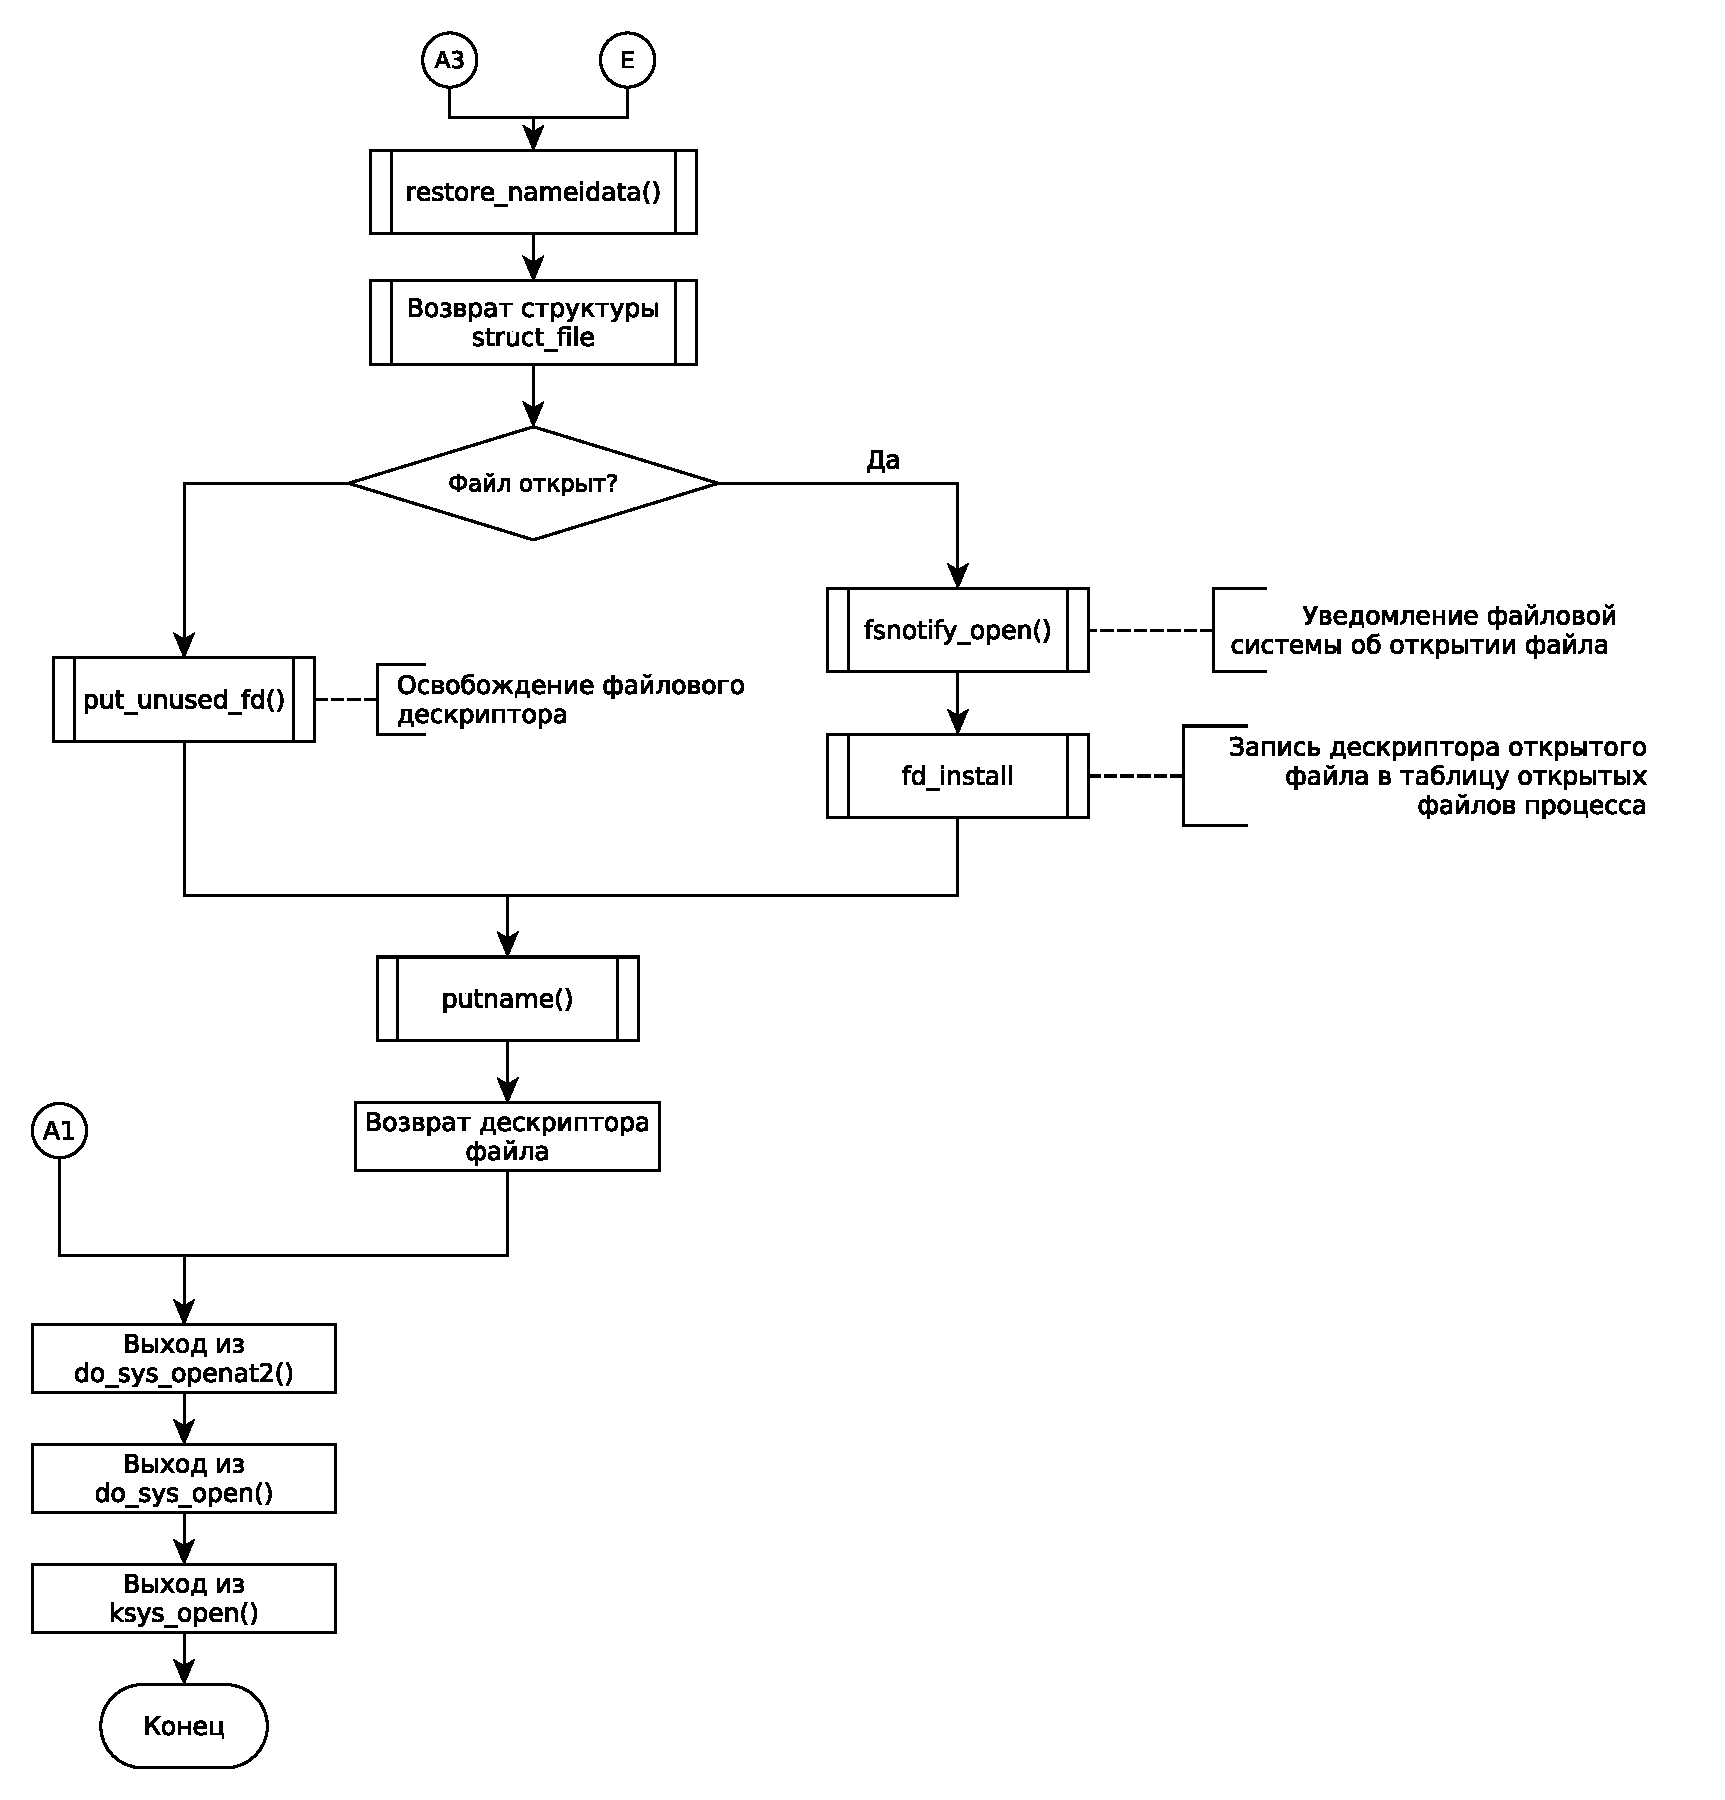
\includegraphics[scale=0.35]{data/image/end.png}
    \caption{Скриншот результата работы команды insmod.}
\end{figure}
